\documentclass[10pt, a4paper, oneside]{scrbook}
\usepackage{fancyhdr}
\usepackage{lastpage}
\usepackage{graphicx}

\graphicspath{ {./img/} }

\title{Shipwars Online}
\author{Group 4}
\date{December 2015, 3. Semester}

% Redefine the plain page style
\fancypagestyle{plain}{%
  \fancyhf{}%
  \fancyhead[L]{University of Southern Denmark\\3. semester, Software Engineering}
  \fancyhead[R]{Project group 4\\11/9 - 2015}
  \fancyfoot[C]{Page \thepage\ of \pageref{LastPage}}%
  \renewcommand{\headrulewidth}{0.2pt}% Line at the header visible
  \renewcommand{\footrulewidth}{0.2pt}% Line at the footer visible
}

\begin{document}

\maketitle

\frontmatter
\tableofcontents
\listoffigures

\input{tex/abstract}


\section{Preface}
The following report is the documentation that describes how the software was developed and why the group made the choices it did. It has been written in connection to with the bachelor degree in software engineering on the University of Southern Denmark - 3. Semester. The project has been developed as a part of the course “Design of software systems in a global context”. The group would like to thank Claudio Giovanni Mattera for the help and advice giving during this project.
\\
\\
This report should be read chronologically to ensure the full understanding of the subject and the choices made by the group.
\\
\\
By signing below here, the group members confirm that they all have been active in and contributed to, the project.
\\
\\
\\

\noindent\rule{10cm}{0.4pt}                                                                  Date: 18/12/2015.
\\
\\
\\
\noindent\rule{10cm}{0.4pt}                                                                 Date: 18/12/2015.
\\
\\
\\
\noindent\rule{10cm}{0.4pt}                                                                 Date: 18/12/2015.
\\
\\
\\
\noindent\rule{10cm}{0.4pt}                                                                 Date: 18/12/2015.
\\
\\
\\
\noindent\rule{10cm}{0.4pt}                                                                 Date: 18/12/2015.
\\
\\
\\
\noindent\rule{10cm}{0.4pt}                                                                 Date: 18/12/2015.


%\input{tex/redaktionelt}

\mainmatter

%
\section{Project Introduction}

	This semester’s project definition was more open than the last
	 two semester projects. We only had to make a distributed system.
	  So we were free choose a topic, as long as it included a client,
		 a server and a database, which were all connected to make an application.
	\\
	\\
	The project handbook actually gave a case where we could develop
	 a system that would help newly started firms make their way into
	  China’s market for production. We decided that we wanted to
		make something else, so we started brainstorming about what
		 each of us wanted to make, then we all came to the agreement
		  of making a game. After that we brainstormed again, this time
			 about what kind of game we wanted to make. It ended up with
			  the classic board game “Battleship” that we would make into
				 a digital version called “Shipwars”. The game fit the criteria
				 perfectly for the requirements we needed. It could have a client
				 that connects to a server that also have a connection to a database
				  where user data is stored. The game would also fulfil our courses
					requirements on this semester project with things like encryption on
					 user data and a market analysis for the cross culture
					  management course. With this game we would eliminate
						the need for being together in the same room when playing, and
						 instead open the possibility to play against people across
						 the globe.
	\\
When we agreed upon the game and its topic, we had to write a project
formulation, and decided to write about the background of board games.
	\\
	\subsection{Project Formulation}

	As board games are rooted in the physical world, board games are limited
	 to the people who can play against each other locally. In order for
	 physical board games to connect a larger player-base that can play anywhere
	  anytime, the Internet may be necessary in order to make it available
		 worldwide. This creates certain problems and here are the ones the
		  group will focus on solving:
	\begin{itemize}
		\item How to digitize a board game?
		\item How to connect multiple people via the Internet?
		\item How to differentiate between the players?
	\end{itemize}


%\input{tex/baggrund}


\section{Requirements}

This chapter is used to explain the thoughts on the requirements that
 were made for the project. This covers analyzing what is involved in creating
  a game. The scope for the project will be covered and finally the use cases
   for the project will be introduced and explained.

\subsection{Game Development Analysis}

The following analysis covers games and gaming split into two parts.
The first part covers the concept of games. The second part covers the
issues with game development.\\\\
The concept of a game can be seen as a goal-oriented experience,
where a group of various activities is played out by one or more players.
These activities are to provide a form of enjoyment or pleasure through
 competition either with oneself or others. In order to keep the game
  consistent rules are imposed onto the game.
In this way, a game employs interactivity and participation of a user,
referred to as a player. The player is put into a scenario with rules and
 goals, where the scenario could be either a reference to or abstraction of
  a realistic situation. The player either gets a goal provided by the game,
   or the player creates their own goal. The goal must be completed to “win”
    the game. Getting into a position of inability or failure to complete the
     goal results in “losing” the game.\\\\
Developing a game can bring certain issues. One of those issues is
 presentation. If the player cannot effectively interact with or understand
  what they are seeing or reading, their experience may not lead to enjoyment.
   Another issue is interaction. Without the proper options to complete the
    required goals, the player may not be able to fulfill the goal. This can
     again lead to an undesirable experience. A third issue is efficiency. If
      the game is unplayable because of inefficiencies, or stability issues,
       the player may not even want to play the game.

\subsection{Scope}

The game will contain an online access functionality that utilizes
 a client-server structure connecting with a database, as the game will
  make use of user accounts for the client, it will be necessary to encrypt
   all user account information. The group choose to use .NET as the
    framework for developing the client-server structure, since C\# is used
     for programming. \\
The game will be very limited in graphics and aesthetics, since the
 focus of the development is on the technical aspects. The group have
  therefore chosen to limit the game to 2D graphics with very simple
   turn-based functionality, and make our own version of the classic
    board game Battleship. The group decided to make the game multiplayer
     to fulfill the distributed system part of the project.

\subsubsection{The Board Game}

The board game “Battleships” is build up around a basic turn based game,
with a grid size of 10x10. Before the game starts each player chooses the
 spot for each of their five ships. Each round a player chooses a coordinate
  to which he attacks from his side to the opponent side. If it is a hit, the
   opponent places a red pin in the boat that is a hit, and the same does the
    player who fired. If it is a miss, the firing player must place a white
     pin in the coordinate to show that the shot did not hit. Each player
      then have five ships in varying sizes up to five pins long. When a
       ship has been sunk the opponent must say what kind of ship that is
        down. When one of the players have lowered all the opponent's
         ships, they win.

\subsubsection{The Computer Game}

The computer game will incorporate the board game’s functionality,
 and make most of it automated. In the first round each player places
  their ships location on the boards’ grid. In the next rounds until a
   player has won, the players will switch turns when a tile has been
    chosen. During the current player’s turn, that player will be shown
     a larger version of the opponent’s grid with their ships locations
      hidden. The player will then choose a tile on the grid to reveal
       whether or not there is a ship. If there is a ship, the tile will
        be marked in red, if not the tile will be marked in gray. A player
         has won when all of the opponent's ships have been fully revealed.

\subsection{Use Case Diagram}

The use cases made for the project were assigned a category in order to
 differentiate between them. The categories were assigned after where the
  use cases’ functionality were most prevalent. UC means the code made for
   the client layer, US for server and lastly UD for database.

\subsubsection{Actors}

\textbf{Player}: Will be interacting with the system though the client.\\
\textbf{Client}: Software part that is responsible for the GUI and the connection
 to the Server. \\
\textbf{Server}: All the software logic will be located here\\
\textbf{Database}: Here the data will be stored.

\begin{figure}[h]
\centering
\includegraphics[scale=0.5]{usecase}
\caption{Usecase diagram}
\end{figure}
\clearpage

\subsection{Use Case Priority}

In order to prioritize our use cases, the group focused on three factors:
 First the amount we were going to learn from realizing the functionality
  involved. Second how important the use case is for fulfilling the
   requirement of the project. Lastly how important the functionality
    is for the final product, if some function is required in another
     use case as well. The more of these criteria, the use case fulfills,
      the higher it is prioritized.

\begin{figure}[h]
\centering
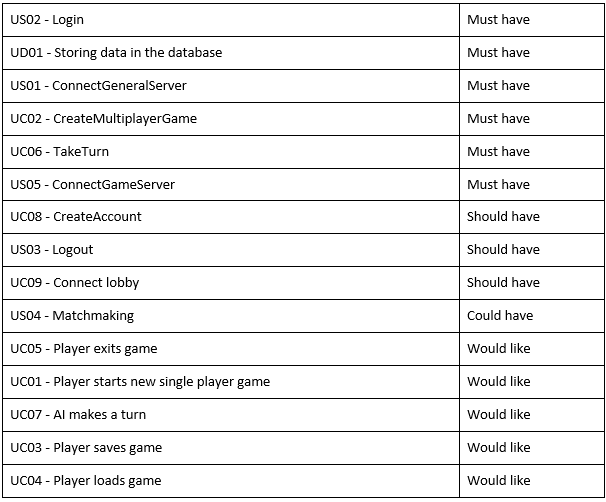
\includegraphics[scale=0.7]{Priority}
\caption{Usecase priority}
\end{figure}
\newpage
\subsection{Use Case Description}
The report will be focusing on 2 use cases to show an idea of the thoughts
 behind the process.

First one will be the creation of a game\\

\begin{figure}[h]
\centering
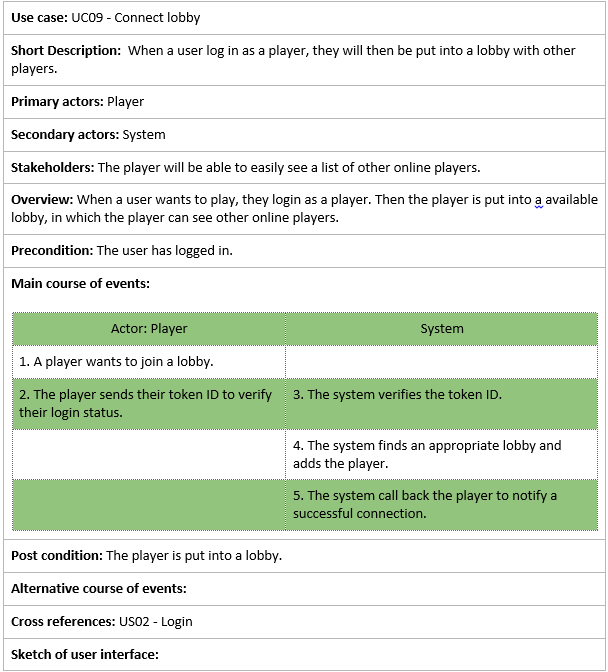
\includegraphics[scale=0.8]{usecon}
\caption{Usecase description for UC09}
\end{figure}
\clearpage

Second one is when the game is started and the player makes a turn.\\

\begin{figure}[h]
\centering
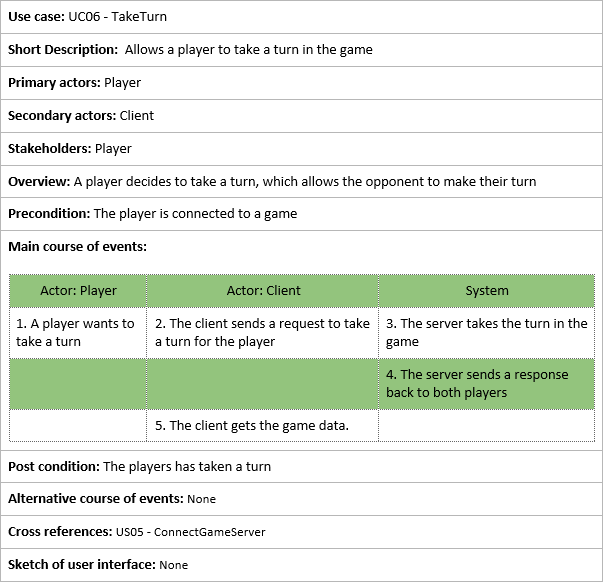
\includegraphics[scale=0.8]{usetak}
\caption{Usecase description for UC06}
\end{figure}
The remaning can be found in the appendix \ref{appendix:useCase_specification}



\section{Tools}

This chapter will go through all the software
used in the project.

\subsection{Development tools}

These are the software used directly for developing
 the software

\subsubsection{Git}

Git is a widely used version control system,
 used by project groups to collaborate as a
  team. When used it creates a repository,
  which makes a history over the changes to
  make it possible to rewind to an earlier
  stage. This was used as the version control
  system for the project.
\subsubsection{Github}

Github is a git server hosting service. It
 makes a server host a git repository available
 for a team to work on. Most of the hosted
 projects are made available to the public
 as an open source project for others to
  explore and give feedback on. This was used
as the host service for our git repository.

\subsubsection{Visual Studio}

Visual Studio is one of the most used IDE’s for
 programing a broad range of programming
languages. It was used in this project to
 make all the C# code the final product
  consists of.

\subsection{Project Management}

These were the software used for managing the task present in the project.

\subsubsection{Trello}

Trello is a time management website used to create a virtual to-do list. When
 a board is created for the team all the members will be able to contribute to
  the board. It was used as the tool to manage our project’s development cycles
   and divide the different use cases equally between the groups.

\subsection{Modelling Tool}

This where the tools used to create artifacts for the project.

\subsubsection{Draw.io}

Draw.io is an online diagram tool able to collaborate with different cloud
 services. The diagrams created here can be shared with the team, allowing
  multiple people to edit

\subsection{Text Editor}

This were the tool used for creating the documentation created during
 the project.

\subsubsection{Latex}

 LaTeX is a document modeling language. It allows the user to design
  a document from scratch in plain text. When the document is done it compiles
   the plain text into the finished text file. This is the tool used to create
    the final report as it provides a high level of control over the fine
     details like layout, design and formatting.

\subsubsection{Google Docs, Google Drive and Microsoft Word}

These were used to make and share documents in the group during the
 development, in a less formal way. Google Docs was our primary text
  editor, where Word was used for assignments.



\section{Methods}

In this section the methods used in the project will be explained and why they were used.

\subsection{Unified Process}

We used UP as a guideline for the project as a whole, which means
that Scrumban was our main structure for the project, and during the
start of the project the inception phase of UP was used when we created
 the inception document.

\subsection{Scrumban}

This is an agile method for creating a product. It is a hybrid
between Scrum and Kanban, utilizing the best of both methods. It
 combines the sprint iteration style from scrum with the bucket list
  and whiteboard planning style of Kanban. It works by putting all the
   requirements for the project onto sticky notes. This then becomes the
    backlog for work, and when a scrum sprint starts the requirement is
     evaluated by its importance. This helps to prioritize the task for a
      given sprint. There is also a limit on how many requirements that can
       be worked on at a given sprint, which will help to make sure that
        resources are not spend unnecessarily and the tasks get done.


%\input{tex/arkitektur}

%\input{tex/design}

%\input{tex/implementation}

%\input{tex/test}

%\input{tex/markedsanalyse}

%\input{tex/diskussion}

%\input{tex/konklusion}

\backmatter

%\input{tex/appendiks}

\end{document}
